\graphicspath{{Chapter1/Chapter1Figs/}}

\chapter{Introduction}
\label{chap:Introduction}

\section{Motivation}
\label{sec:Motivation}
The insulin/insulin-like signalling and Target of Rapamycin (IIS/TOR) network is a central regulator of cellular growth and metabolism and plays an important role in ageing and age-related diseases. In response to metabolic stimuli such as insulin, nutrients or energy, a cascade of signalling events modulated by post-translational modifications, in particular phosphorylation, occurs to promote TOR activity. Once phosphorylated, TOR governs cellular processes essential for development and ultimately ageing, such as promotion of cell growth, proliferation and metabolism, improvement of mitochondrial function, and inhibition of autophagy and apoptosis. Hence, understanding the functional mechanisms of the IIS/TOR network is an essential component in extending our knowledge on ageing and age-related diseases.\\
The increase of \emph{in vitro} data collected to extend our knowledge on its regulation and consequently improve drug intervention, has notably highlighted the complexity of the mTOR network. This complexity is also increased by the intrinsic time-dependent nature of cellular regulatory networks cross-talks and feedbacks. This high level of complexity found in many biological signalling pathways raised interest for systems biology in the scientific community. Systems biology constitutes a powerful tool for mathematically formalising biological networks and investigating their dynamical properties. In this work, the regulatory mechanisms of the mammalian TOR network were investigated in detail using a combined \emph{in silico}-\emph{in vitro} systems biology approach.

\section{Objectives}
\label{sec:Objectives}
In the first two years of my doctorate, I developed two computational models of the TOR signalling network that further our understanding of the influence of growth factors and nutrition on cellular decisions. Calibrated on immunoblot-based experimental data, provided by the team of Kathrin Thedieck, Freiburg University, Germany, these models were used to investigate and test hypotheses of activation of mTOR Complex 2 and AMPK. As mTOR and AMPK are important regulators of FoxO and autophagy, understanding their functional mechanism represents a crucial aspect in ageing.\\
In the last year of my doctorate, I developed a mathematical model which integrated knowledge from several biochemical processes of interest in ageing research. Through the interaction with the team of Professor Thomas Von Zglinicki, Institute for Ageing and Health, Newcastle University, UK, a new process-oriented modelling project was begun with the aim of combining behaviours of some of the most studied components in ageing research: insulin/TOR, ROS, FoxO and mitochondria. This work aimed to establish the first mathematical extended framework for cellular senescence. At this initial stage, my main objective was to formally provide a mechanism for explaining the transition of cell state from normal to senescent.\\
By investigating systems dynamics with detailed \emph{in vitro} time-course experimental data and network modelling with a focus on functional outcomes at the cellular level, these projects contributed to a better understanding and opened new avenues for future research on TOR signalling in development and ageing and for therapies of age-related diseases.

\section{Outline}
\label{sec:Outline}
This thesis follows a tree structure based on a TOR-focused introduction on ageing, insulin/TOR network and systems modelling, and three systems biology projects (see Figure \ref{fig:outline}).\\
In Chapter \ref{chap:TOR in ageing and age-related diseases}, a general introduction on ageing and the recent implications of TOR in ageing and age-related diseases are presented in order to contextualise this work inside a theoretical framework. \\
In Chapter \ref{chap:mTOR network: an overview}, the insulin/TOR network is discussed from a molecular biology perspective. In this chapter the upstream and downstream signalling pathways of both mTOR Complex 1 (mTORC1) and mTOR Complex 2 (mTORC2) are extensively described.\\
Chapter \ref{chap:Systems biology for investigating mTOR network in ageing} introduces systems biology in the specific case of dynamical models optimised over experimental data sets as well as the most prominent analyses from dynamical systems theory. A review of the recent published mTOR mathematical models is proposed in order to link systems modelling with TOR biology.\\
Chapter \ref{chap:A dynamical network model of mTOR signalling reveals TSC-independent mTORC2 regulation} describes the differential investigation of three hypotheses of mTORC2 activation and the discovery of a new class I PI3K independent of p70-S6K-negative feedback loop, which promotes mTORC2 activity upon insulin stimulation. The article related to this work and published in Science Signalling is attached in Appendix \ref{appendixA}. \\
In Chapter \ref{chap:A modelling-experimental approach reveals IRS dependent regulation of AMPK by insulin}, the previously described model was extended with the inclusion of AMPK regulation. Using a hypothesis ranking approach based on model goodness-of-fit, AMPK activity was \emph{in silico} predicted and \emph{in vitro} tested to be activated by the insulin receptor substrate (IRS) upon insulin stimulation. The article related to this work and published in FEBS Journal is attached in Appendix \ref{appendixB}. \\
Chapter \ref{chap:A dynamical mTOR-ROS model for cellular senescence} discusses a new mathematical model linking mTOR with the oxidative stress response, mitochondria regulation, DNA damage through FoxO transcription factors and Mfn2. This work provides the formalisation of a dynamical mechanism to explain the state transition from normal to senescent cells and their irreversibility.\\
Finally, a general conclusion of this thesis is presented in Chapter \ref{chap:Conclusions and outlook}.


\clearpage

\begin{figure}[tb]
	\begin{center}
		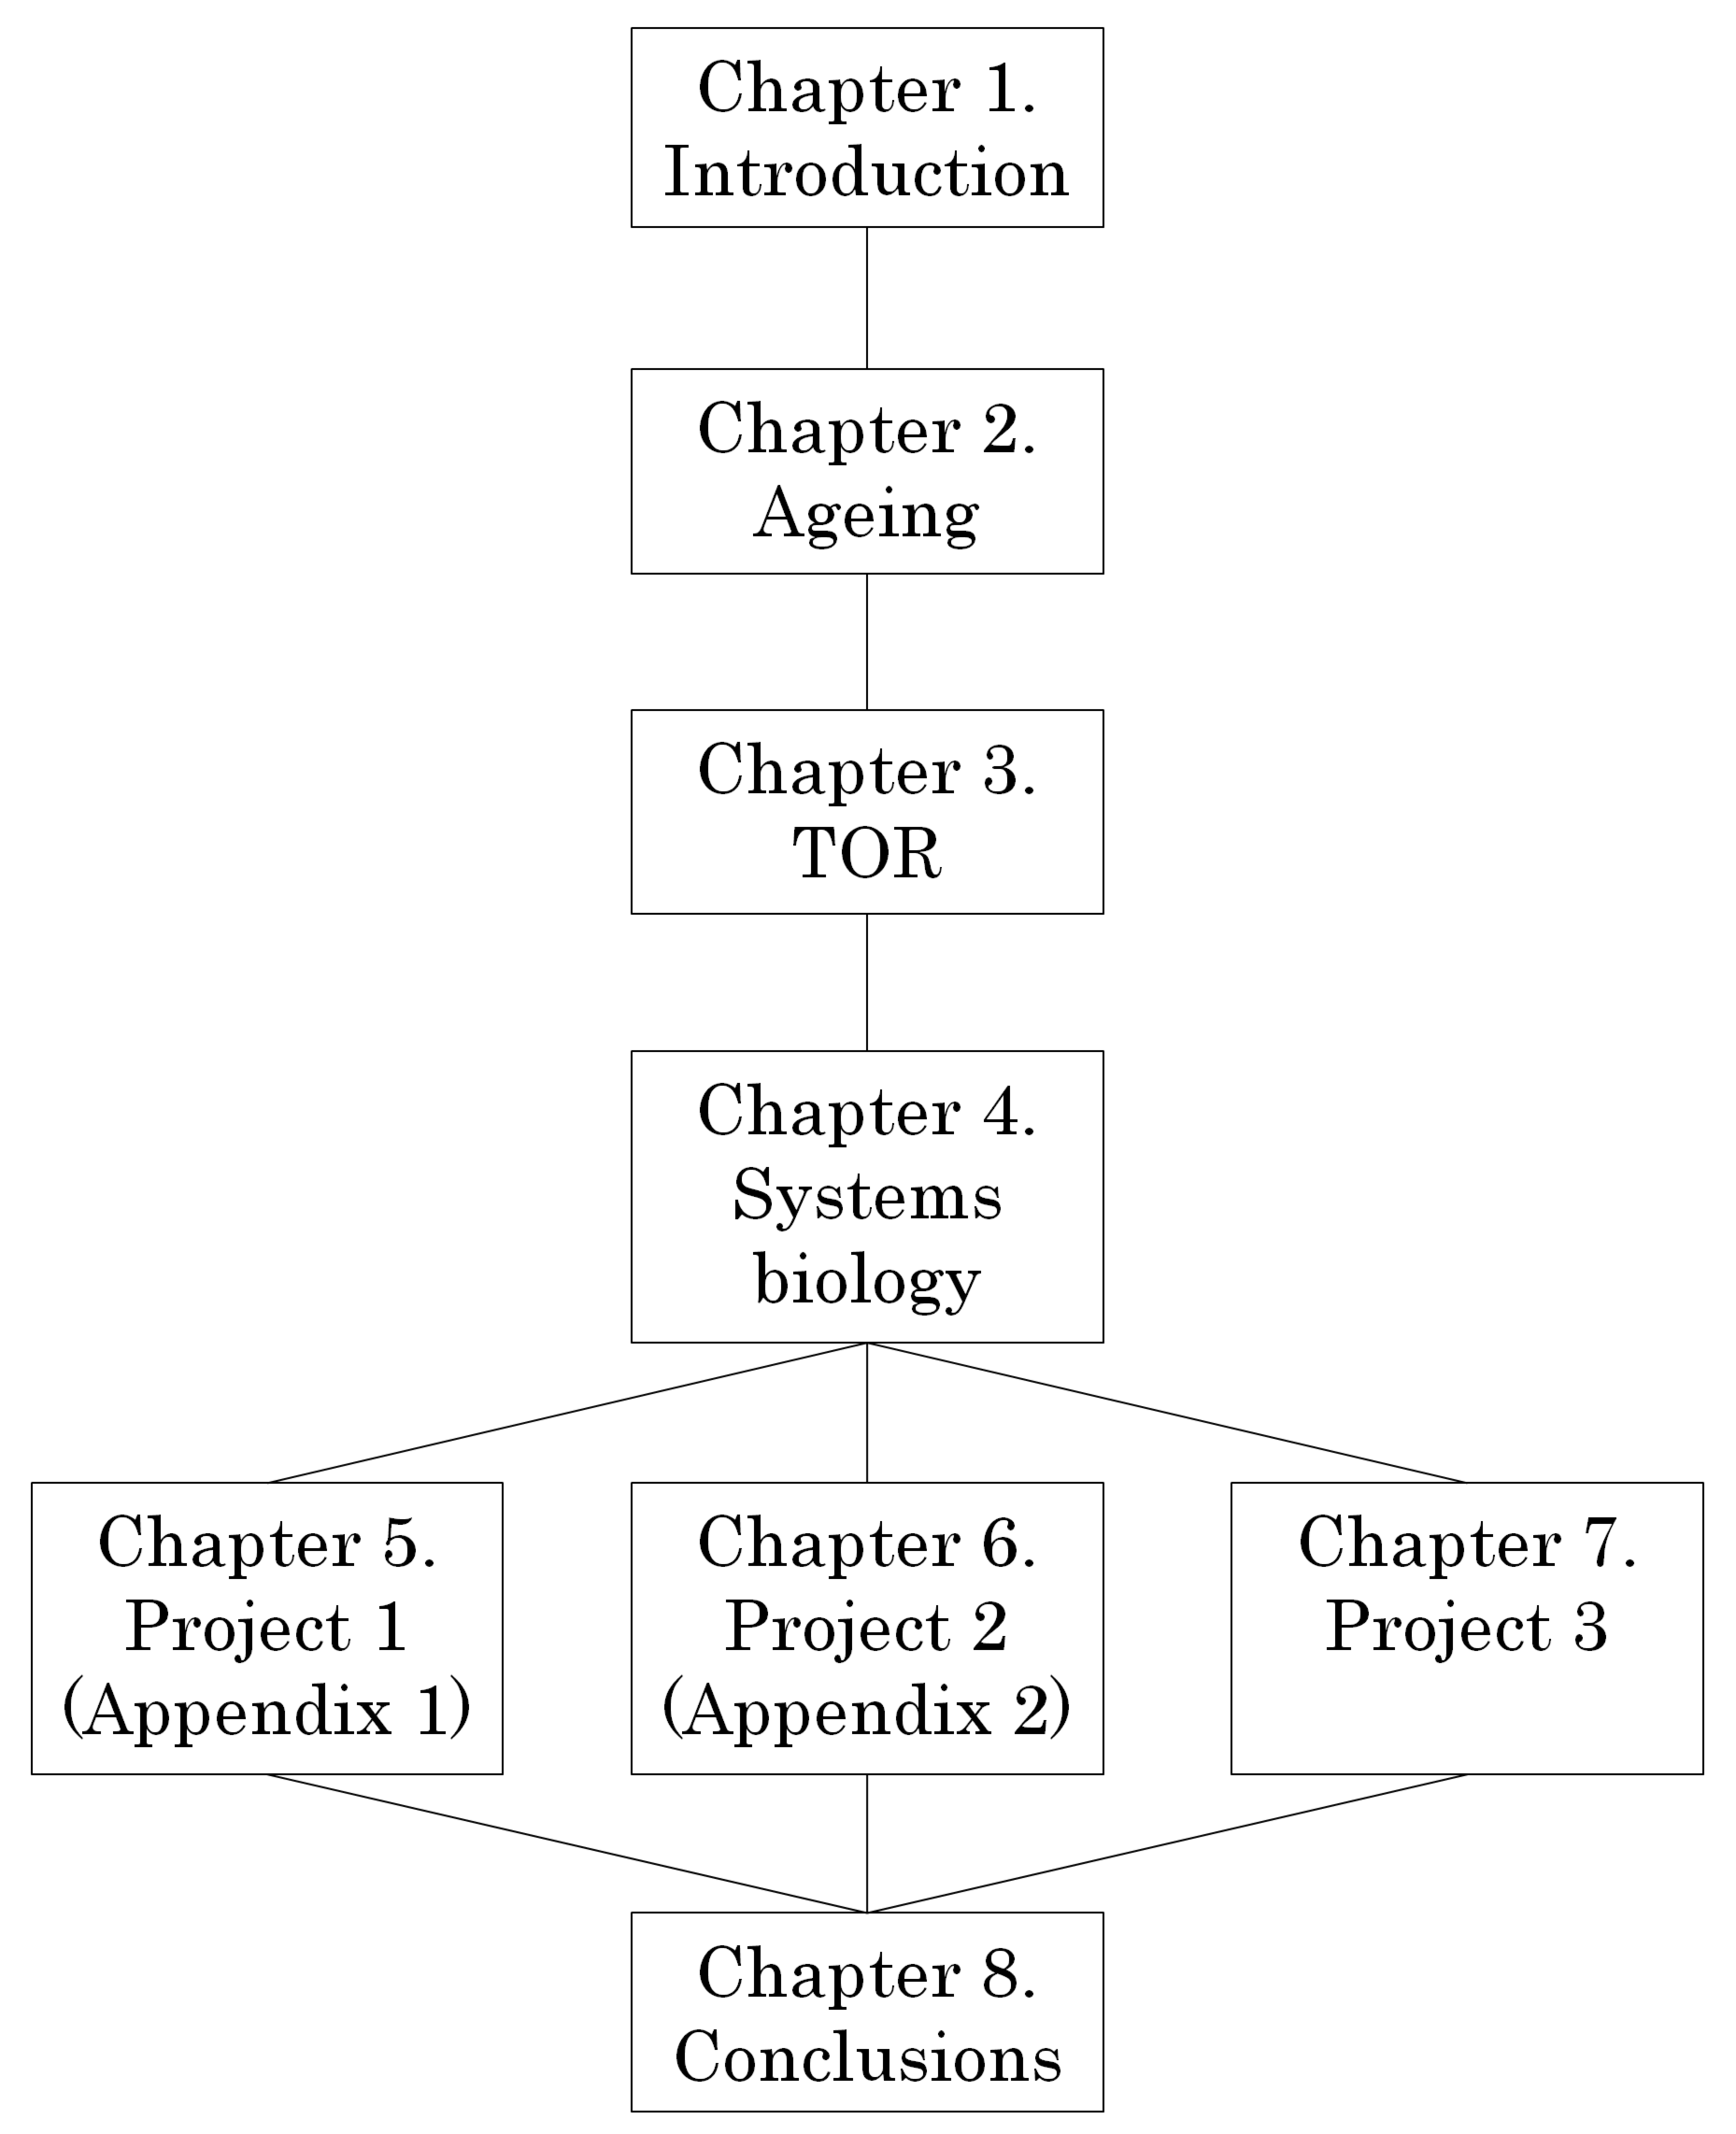
\includegraphics[width=5.0in]{outline.png}
		\caption[Thesis structure]{Thesis structure.}
		\label{fig:outline}
	\end{center}
\end{figure}
\clearpage





%%% ----------------------------------------------------------------------


%%% Local Variables: 
%%% mode: latex
%%% TeX-master: "../thesis"
%%% End: 
